\chapter{Snapshot}
\label{chap:snapshot}

    One of the major features in the Kabi File System is the writable copy-on-write snapshot. A snapshot is a point-in-time copy of a defined collection of data \cite{snapshot_def}. A read-only snapshot is an immutable copy of the file system data at a time spot, while a writable snapshot can be considered as a writable fork of such copy. Snapshot nodes are designed as a basic type of component in the Kabi File System. The ``current'' view of the file system is also treated as a writable snapshot (the latest snapshot in default branch). This snapshot system focuses on reducing the storage space occupied by a snapshot.

    According to the Storage Networking Industry Association, three classic snapshot approaches include split-mirror, changed block, and concurrent~\cite{snapshot_types} The split-mirror approach copies every byte from source to snapshot. The process is time consuming hence it usually requires planning in advance. The changed block approach applies the copy-on-write strategy on the snapshot. The concurrent approach redirects IO requests to different storage spaces associated with snapshots. Instead of making a copy and overwriting the copy, write IO requests will be redirected to a separate storage space. While read IO requests may be redirected depends on whether the data has been changed since last snapshot.

    Our snapshot system uses a strategy that is a mixture of copy-on-write and redirect IO. It uses the enhanced copy-on-write strategy on the actual data and the redirect IO strategy on metadata. In our snapshot system, all snapshots (except for one) log the changes since the prior snapshot. Such that the snapshot system can then recover the content of the snapshot based on the previous snapshots and the log of changes, as shown in \fref{fig:snapshot_patch}. The only exception is a special snapshot called the ``head snapshot'' which references the content of the entire file system. Other snapshots are called referencing snapshots. They contain a reference to another related snapshot and an array of patch objects. Each patch object in the array reflects a series of changes on a single file or a single directory since the prior snapshot.

\begin{figure}[t]
\centering
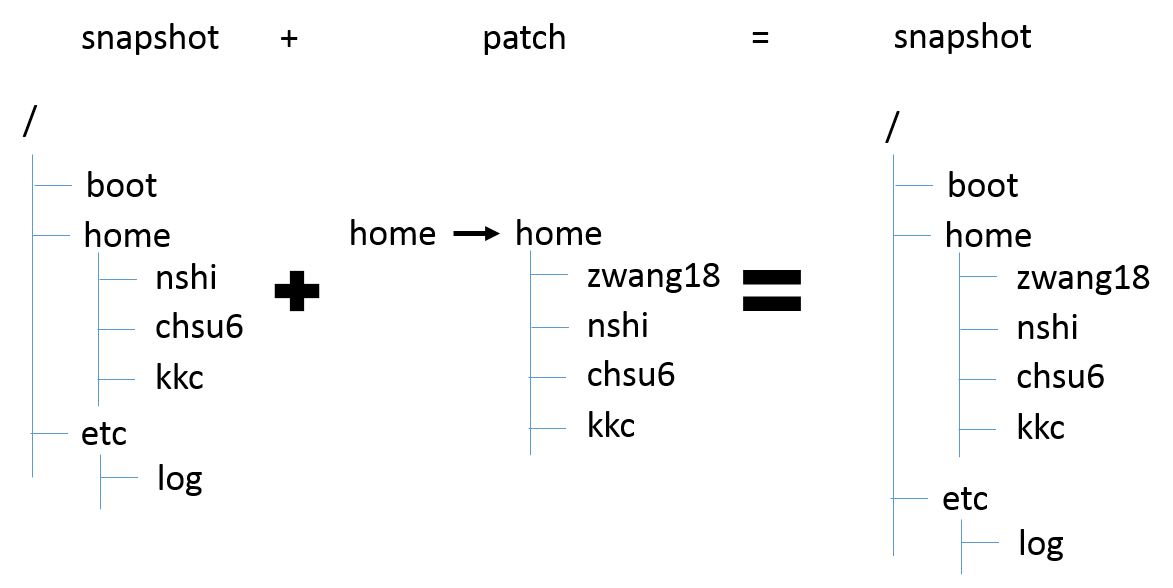
\includegraphics[width=0.8\textwidth]{Chapter-4/figs/fig23.png}
\caption{Snapshots and Patches}
\label{fig:snapshot_patch}
\end{figure}

\section{The Snapshot Tree}

    The snapshot system in the Kabi File System uses an approach based on patches. A similar approach that is adopted by ext3cow uses a reserved field in inode to reference the previous version of inode, as shown in \fref{fig:snapfs_approach}. One advantage of the patch based approach is that it supports the tree structured snapshots and the writable snapshots. With tree structured snapshots, one can fork the file system keep multiple ``current'' version of the file system at the same time.

\begin{figure}[t]
\centering
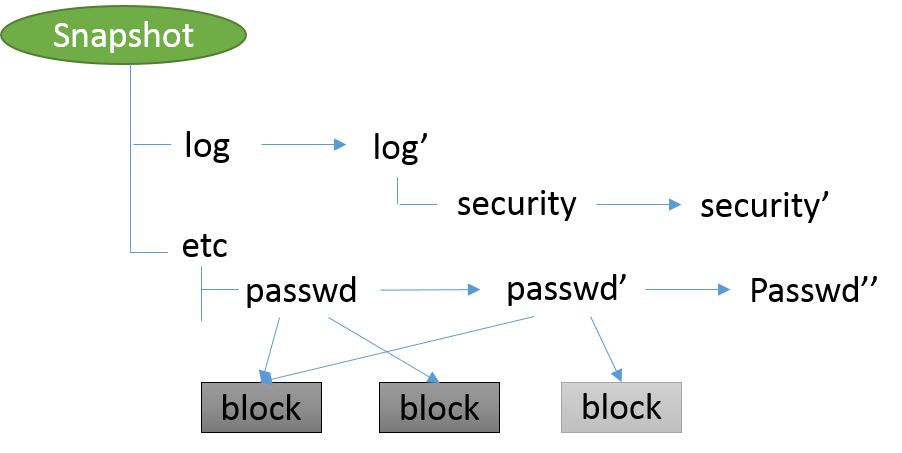
\includegraphics[width=0.7\textwidth]{Chapter-4/figs/fig24.png}
\caption{Snapshots in SnapFS}
\label{fig:snapfs_approach}
\end{figure}

    Snapshots in the Kabi File System are represented by snapshot nodes and these nodes form an up-tree. In an up-tree, every child points to its parent. \fref{fig:snap_tree_example} shows an example of a snapshot tree. The right bottom node (node H) is the root of the tree. The root of the snapshot tree is always the head snapshot.

\begin{figure}[t]
\centering
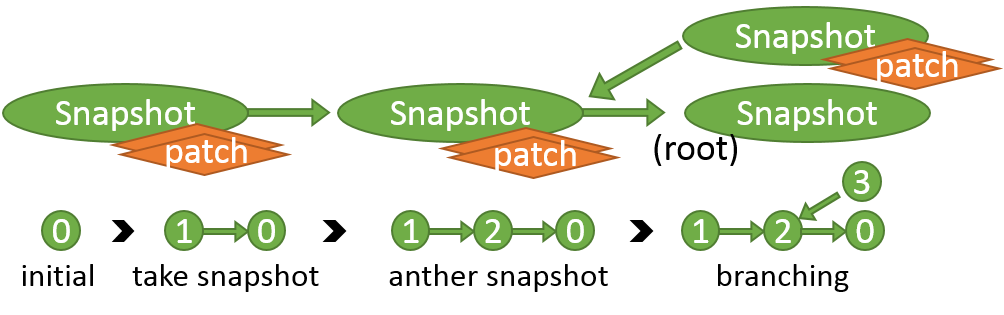
\includegraphics[width=0.8\textwidth]{Chapter-4/figs/fig13.png}
\caption{An Example of Snapshot Tree}
\label{fig:snap_tree_example}
\end{figure}

    Initially, the file system contains a default writeable snapshot node (node H in \fref{fig:snap_tree_example}) representing the current view of the file system. This special snapshot called the head snapshot is the root of the snapshot tree and the only snapshot node that does not reference other snapshot. For initial state,  writes to the file system go directly into the head snapshot.
    
    After a snapshot is taken, a new snapshot node (node 1 in \fref{fig:snap_tree_example}) is created referring to the head snapshot node. Subsequent write operations will not only write data into the head snapshot but also submit patches to all snapshot connected to head snapshot, so as to reflect the difference between snapshot node 1 and its referencing node H.

    Branching a snapshot creates a writable copy of an existing snapshot. The branching operation is implemented by creating a new snapshot node referring the snapshot being forked. As shown in \fref{fig:snap_tree_example}, node 3 (the writable copy) is created and connected to snapshot node 2 (the existing snapshot) in order to fork the file system based on snapshot 2.

    In the snapshot tree, each writable snapshot corresponds to a branch. A branch consists of the writable snapshot (the current status of the branch) and its historical snapshots (the history of the branch). The main branch is the branch where the head snapshot node lies. \fref{fig:branches} shows the idea of branch. In the example, there are two branches in this 5-node snapshot tree. Node H is the root of the up-tree so it represents the head snapshot. Hence node 1, node 2, and node H form the main branch. In the figure, nodes on the left correspond to older snapshots and nodes on the right correspond to more recent snapshots. Therefore in main branch, node 1 is the oldest snapshot while node H represents the latest state. Node 1 and Node 2 form the history of main branch and node H is the current view of main branch. Node 4 is another writable snapshot and it belongs to a side branch. The side branch consists of node 1 (the oldest), node 2 (the second oldest), node 3 (the third oldest), and node 4 (most recent). Note the arrows between nodes reflect the referencing relations between snapshots, not the order of creation.

\begin{figure}[t]
\centering
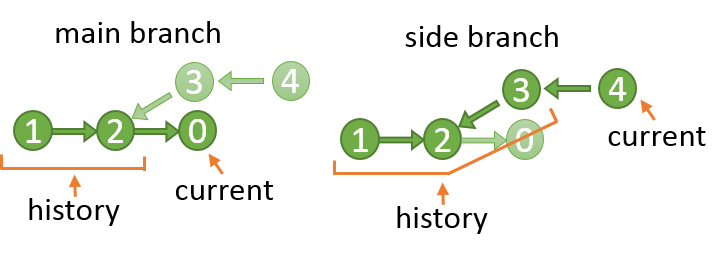
\includegraphics[width=0.65\textwidth]{Chapter-4/figs/fig22.png}
\caption{Branches}
\label{fig:branches}
\end{figure}

\section{Snapshot Nodes and Patch Object}

    As mentioned in previous sections, there are two types of snapshot nodes in this file system, namely the head snapshot node and the referencing snapshot node. The head snapshot is special in the file system. It is the root of the up-tree and does not reference any other snapshots. Instead it stores the entire content of current view in the main branch by referencing the directory node of the root directory. In this way, read access to the head snapshot node is straight forward and faster than any other snapshot. Because of this property, the head snapshot is recommended to be used to represent the most frequently accessed snapshot or the current state of the default branch.

    On the other hand, a referencing snapshot does not reference its own root directory but it keeps a reference to another snapshot node and an array of patch objects. The array of patch objects represent the difference in content between this referencing snapshot and the referenced snapshot. Reading a referencing snapshot will first read the file system content in referenced snapshot and then lookup the patch list to find out if the content has been changed in this snapshot. To write data, the referencing snapshot uploads the changed nodes into the database, build a patch object with both IDs, upload and attach the patch to the snapshot node in the remote machine. This upload and attach process is atomic and it ensures the file system not being left in an incomplete state. Once a referencing snapshot is referenced by some other snapshot nodes, it becomes a read only snapshot. \fref{fig:root_and_nonroot} shows the structure of a head snapshot node (right) and the structure of a referencing snapshot (left).
    
\begin{figure}[t]
\centering
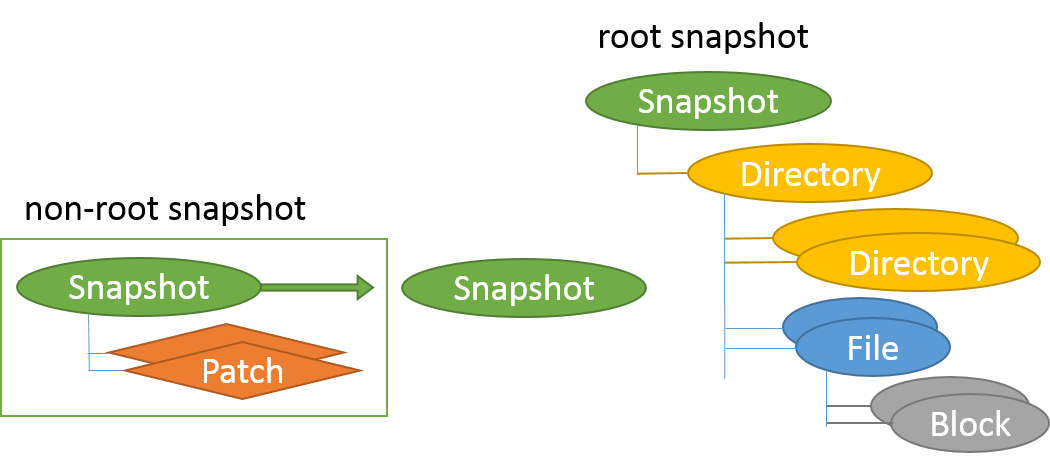
\includegraphics[width=0.75\textwidth]{Chapter-4/figs/fig12.png}
\caption{Root Snapshot and Non-root Snapshot}
\label{fig:root_and_nonroot}
\end{figure}

    A patch object reflects one or more modifications to a single node. The node can be either a file node or a directory node. The patch object references a pair of file nodes or directory nodes. The two nodes referred are the target node (original version) and its replacement (changed version).

    \fref{fig:patches} demonstrates the way the patch system works. Snapshot 1 and 2 demonstrate how a directory changes between snapshots. The directory that is represented by node $d_2$ in snapshot 2 is now replaced by directory node $d_1$ in snapshot 1. In snapshot 2, the directory has a new subdirectory but the file under that directory remains unchanged. Hence the target node (node $d_2$) and replacement node (node $d_1$) have a reference to the same file node but the target node $d_2$ has one more reference to a directory node. In the example of snapshot ($a$) and snapshot ($b$), a file changes in both snapshot, its original version is $f_1$, the intermediate version in snapshot ($b$) is $f_2$ and the final version is $f_3$ in snapshot ($a$). In snapshot $\alpha$ and snapshot $\beta$, file $f_3$ is replaced by $f_2$ in snapshot ($\beta$) and replaced by $f_1$ in snapshot ($\alpha$).  

\begin{figure}[t]
\centering
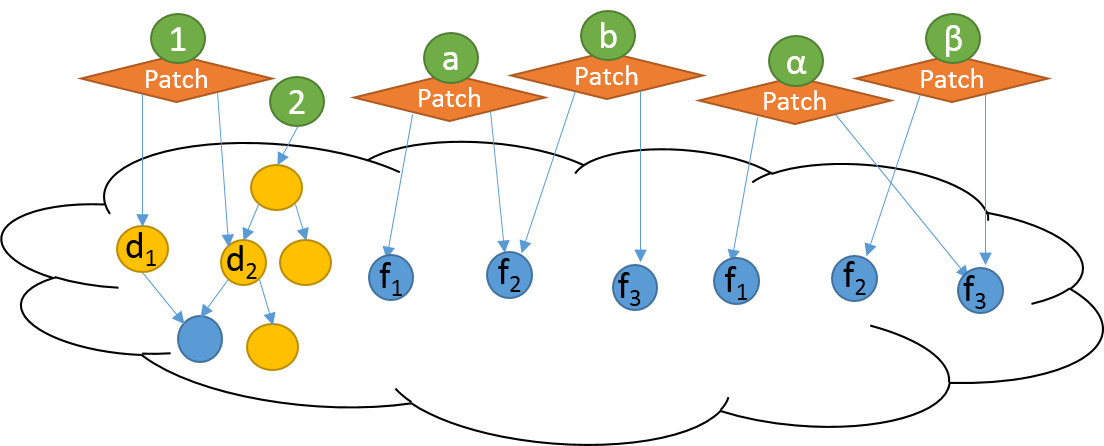
\includegraphics[width=0.75\textwidth]{Chapter-4/figs/fig14.png}
\caption{The Principle of Patches}
\label{fig:patches}
\end{figure}

\section{Snapshot Related Operations}

    Operations in snapshot system read the content in a snapshot and make changes to a writeable snapshot. Making changes to the current view of the file system also involves snapshot write operation as the current view of the file system is also treated as a snapshot in the Kabi file system.

\subsection{Read Operations}

    When reading a file or a directory in a referencing snapshot, the file system must do a large number of lookup operations in patch lists to ensure that the file system is referring to the correct version of the node. For instance, in \fref{fig:read_patches}, to read the file ``/a/d.txt'' in snapshot 1, the file system will first read in the ``/'' directory in the head snapshot which is node 3. Then it transverses all involved snapshots (1 and 2) to see if there's a patch whose target node is node 3. Since no such patch is available, this means node 3 is the ``/'' directory node of all snapshot nodes (1, 2 and 3). Then the file system will look for the ``a'' directory under node 3 and corresponding patches. This time there is a directory (node 9) with the display name ``a'' under node 3 but there is also a patch to node 9 in snapshot 2. That means node 5 is the ``/a'' directory node of snapshot H while node 6 is the directory node of snapshot 1 and snapshot 2. Follow the same procedure, we will find node 8 is the ``/a/d.txt'' node in snapshot 2 but for snapshot 1 ``/a/d.txt'' is represented by node 6.

\begin{figure}[t]
\centering
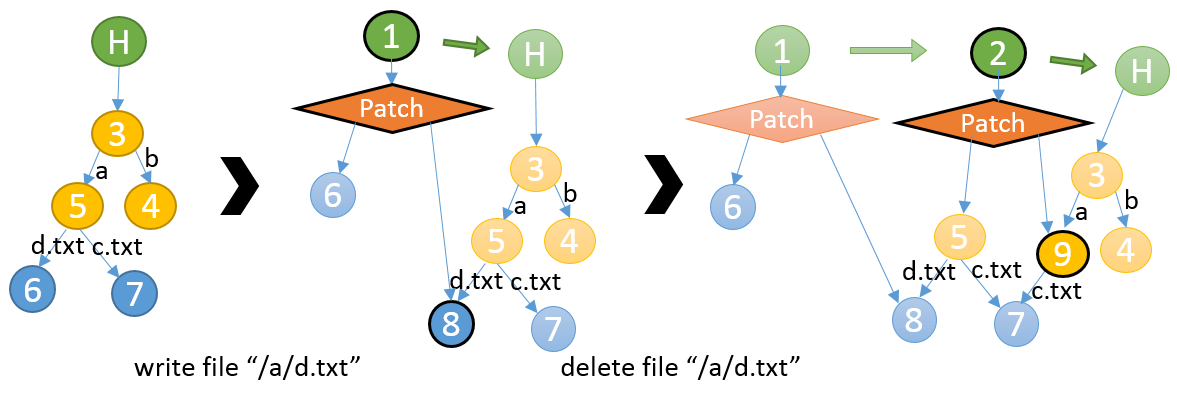
\includegraphics[width=0.5\textwidth]{Chapter-4/figs/fig18.png}
\caption{Read a Snapshot}
\label{fig:read_patches}
\end{figure}

    As one can see, read operations rely on the patch lookup operation. To avoid massive query operations and traverse operations on all involved snapshot and patch objects on every read operation, a local patch list will be built and stored as a hash table in memory when a referencing snapshot node is mounted. The local patch list combines all patches that may be used for a node lookup. In the example shown in \fref{fig:combine_patch_list}, when mounting snapshot 3, a local patch list that contains all effective patches in snapshot 3 and 2 is created.

\begin{figure}[t]
\centering
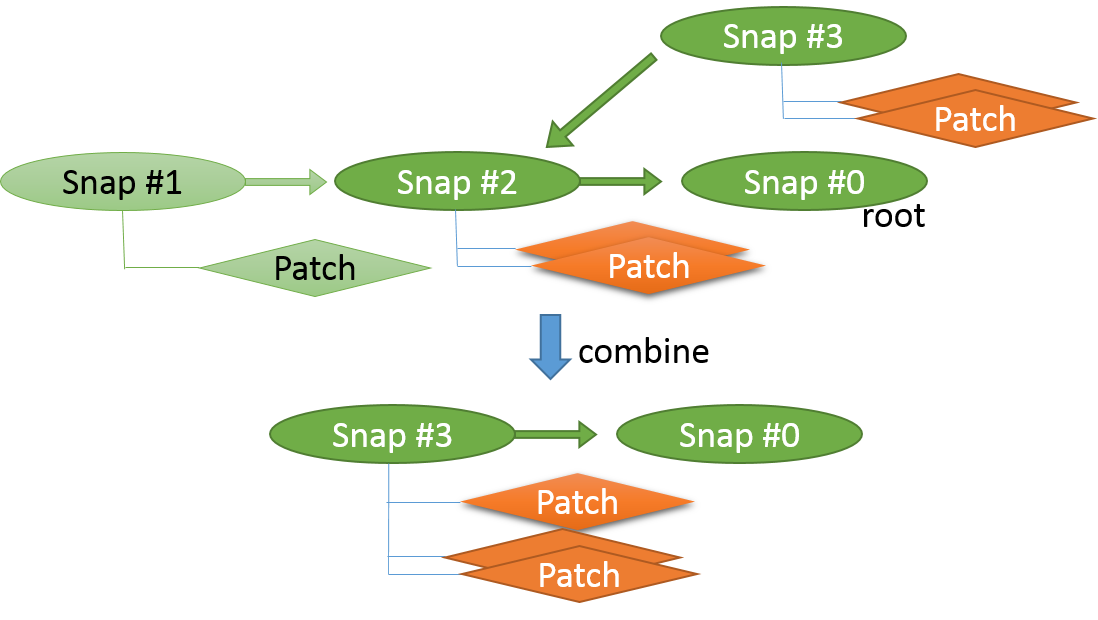
\includegraphics[width=0.8\textwidth]{Chapter-4/figs/fig15.png}
\caption{Combine Patch Lists}
\label{fig:combine_patch_list}
\end{figure}

    Not all patches in patch lists are effective or will be combined into the local patch list. Because patches come from different patch lists, when combining them together, some patches can be merged into one and some are unnecessary. For instance, in \fref{fig:merge} snapshot (a) and (b) the replacement node $f_2$ of a patch is also the target node of another patch, these two patch object can be merged into one local patch. Another example is when reading snapshot ($\alpha$) and ($\beta$), the two patches shown in the figure have the same target node $f_3$. If snapshot ($\alpha$) is mounted, the patch in snapshot ($\beta$) will become ineffective and will be discard when building the local patch list.

\begin{figure}[t]
\centering
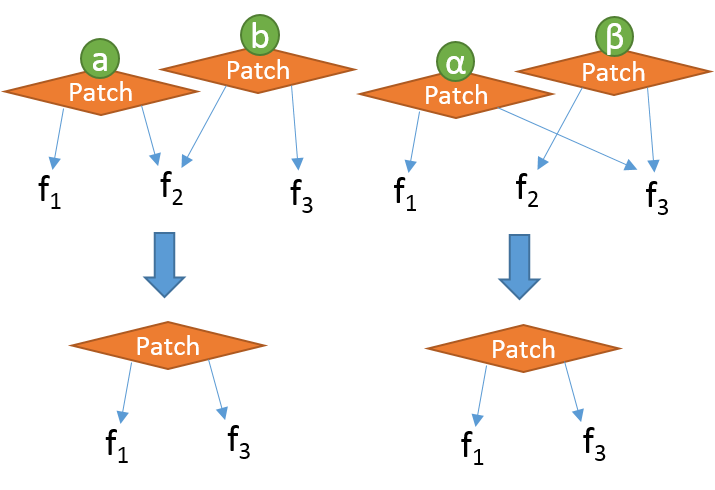
\includegraphics[width=0.7\textwidth]{Chapter-4/figs/fig19.png}
\caption{Merge Patches (Local)}
\label{fig:merge}
\end{figure}

\subsection{Write Operations}

    In both copy-on-write snapshot system and redirect IO snapshot system, a file system entity (block, file, directory) may be referenced for one or more times. The referencer can be snapshots or the ``current'' view of the file system. If an entity is referenced only once, write operation to that entity will be straight forward. This is a write operation within a snapshot. On the other hand, when an entity is referenced more than once, the snapshot system usually needs special treatment to the write operation. Otherwise a direct in-place write will affect all referencers. In the snapshot system, we focus on the latter case. If not otherwise specified, ``write operation'' in this section refers to those write calls whose target entity is referenced more than once.

	\fref{fig:create_snapshots} briefly demonstrates how patch objects and snapshots work with write operations. This example has three snapshots. Node H is the head snapshot node representing the current status of the main branch. Snapshot node 2 represents the initial status and node 1 is the intermediate status of the main branch. Initially, the file system contains three directories ``/'', ``/a'', ``/b'' and two files ``/a/c.txt'', ``/a/d.txt''. In between the initial snapshot and the next snapshot, file ``/a/d.txt'' was overwritten so its representing node was changed by a patch. After snapshot 2 is taken, the file ``/a/d.txt'' was deleted. A new patch was attached to snapshot 2 to reflect this change.

\begin{figure}[t]
\centering
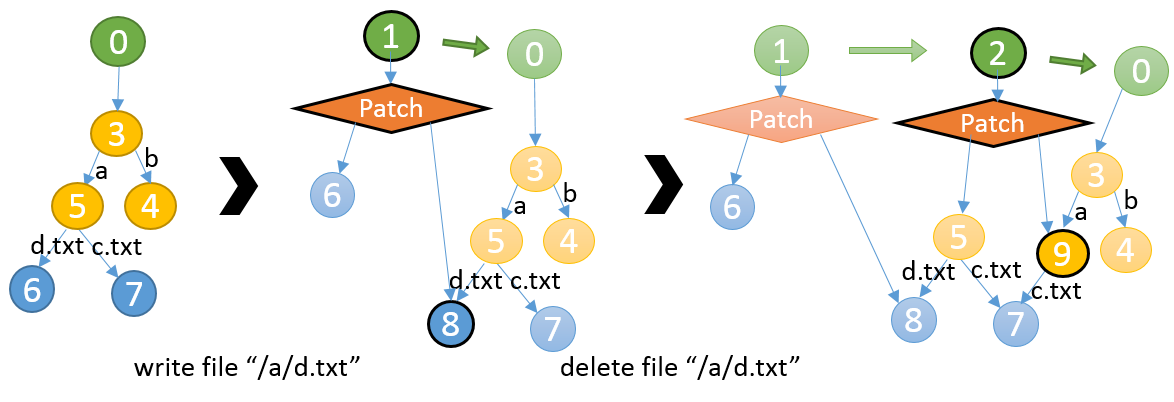
\includegraphics[width=0.95\textwidth]{Chapter-4/figs/fig26.png}
\caption{Example - Create Snapshot after Write}
\label{fig:create_snapshots}
\end{figure}

    \fref{fig:take_snapshot_root} and \ref{fig:take_snapshot_nonroot} show how to take snapshots on the main branch and side branches. In order to take a new snapshot on the main branch, the file system will create a new snapshot node in between the head snapshot and its adjacent snapshot nodes. This newly created snapshot will reference the head snapshot and have an empty patch list. This new snapshot node will represent the status of this branch at the time it is created. The current state of the main branch is still represented by the head snapshot.

\begin{figure}[t]
\centering
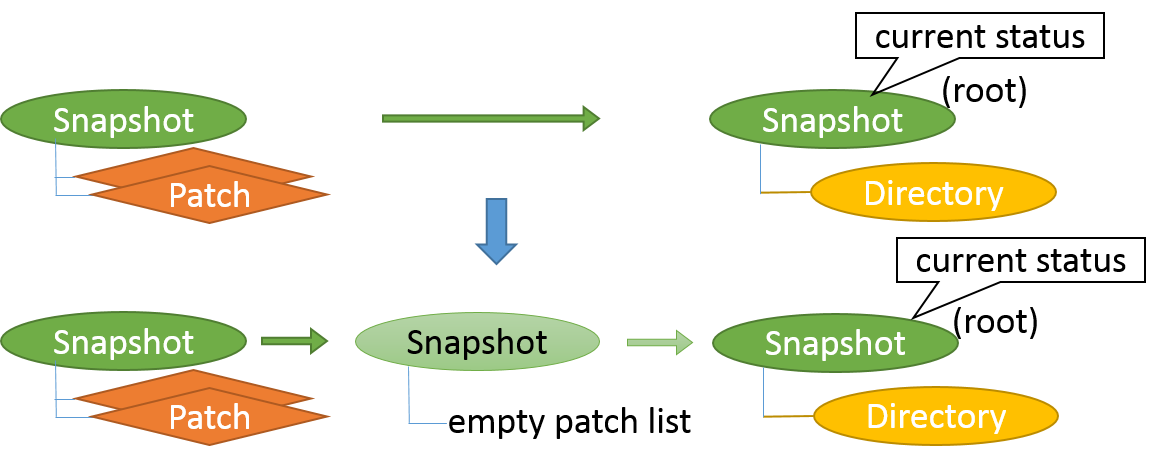
\includegraphics[width=0.8\textwidth]{Chapter-4/figs/fig20.png}
\caption{Take Snapshots on Main Branch}
\label{fig:take_snapshot_root}
\end{figure}
    
	To take a snapshot on a side branch, the file system will create a new snapshot node and attach it to the end of the side branch. The newly created snapshot node will reference the latest snapshot on this branch and have an empty patch list. After attached to the branch, this snapshot will become the current status of this branch.

\begin{figure}[t]
\centering
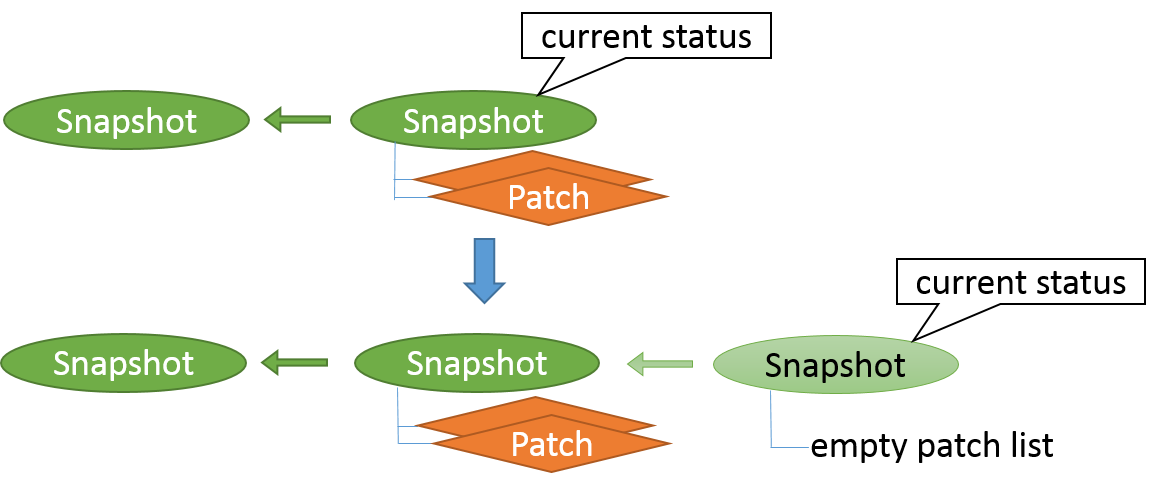
\includegraphics[width=0.8\textwidth]{Chapter-4/figs/fig21.png}
\caption{Take Snapshots on Side Branch}
\label{fig:take_snapshot_nonroot}
\end{figure}
    
    When writing a snapshot other than the head snapshot, the Kabi File System will submit new patches to that referencing snapshot to reflect the change. In the first example shown in \fref{fig:write_snapshot_node}, the file system is writing the head snapshot in the main branch. It is replacing node X with its newer version Y. Node Y will replace node X directly in the head snapshot. In order to keep its previous version ``X'' in snapshot 2, a ``reverse'' patch object (Y-to-X) will be submitted to revert node Y back to its original version X. In this way, the head snapshot will have the new version Y while all other snapshots keep the old version X. In the second example, the file system is trying to replace node X with its new version Y in snapshot 3. Compared to the first example, the file system now can simply submit a X-to-Y patch to snapshot 3. In the third example, we demonstrate a walk-around to write to an internal snapshot node by creating a branch based on that internal node and writing to that branch.

\begin{figure}[t]
\centering
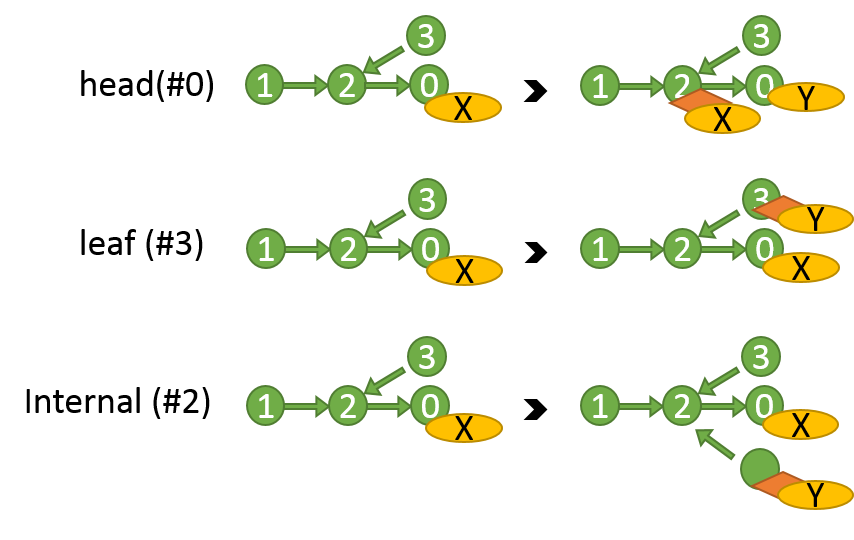
\includegraphics[width=0.7\textwidth]{Chapter-4/figs/fig17.png}
\caption{Write a Snapshot Node}
\label{fig:write_snapshot_node}
\end{figure}

    To create a branch based on the head snapshot, it is recommended to create a dummy snapshot first and then fork from that dummy node rather than branching the head snapshot directly. This is because a write operation to the head snapshot will submit patches to all snapshot nodes connected to the head snapshot node. Hence we wish to limit the number of snapshots connected to the head snapshot. If we fork the head snapshot directly then there will be multiple snapshot nodes connected on to the head snapshot node. \fref{fig:dummy_node} demonstrates this issue. In the upper case, with dummy snapshot node (node 2), a write operation to head snapshot (node 0) only submits a patch to the dummy node. But in the lower case, when there is no dummy node, a write operation to the head node has to submit two identical patches to node 1 and node 3.

\begin{figure}[t]
\centering
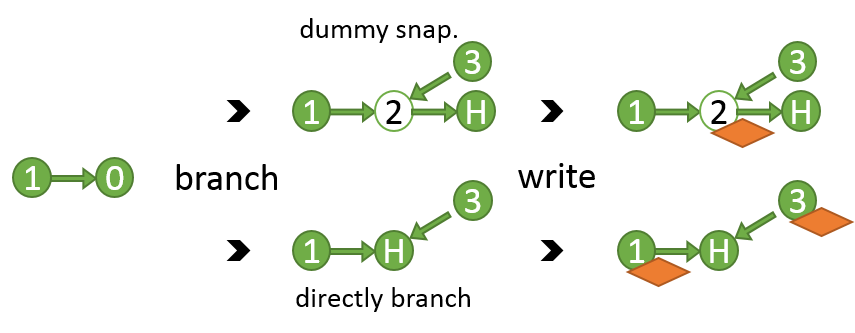
\includegraphics[width=0.8\textwidth]{Chapter-4/figs/fig16.png}
\caption{Branching Root Snapshot Node Directly}
\label{fig:dummy_node}
\end{figure}

	Generally, within one snapshot, each node (file or directory) should have no more than one patch associated with it. For example, a patch replacing node 0 with node 1 and another patch replacing node 1 with node 2 can be merged into one patch. This happens when a node is modified multiple times in one snapshot. For time and space efficiency, it is better to merge them into one patch.
	
\section{Enhancing Copy-on-Write and Deduplication}

	The copy-on-write strategy and file system deduplication improve space efficiency of the file system. File system deduplication finds and eliminates duplicated blocks and files while the classic copy-on-write strategy eliminates unnecessary copy of an unchanged block to snapshots.

\subsection{Motivation}

    A classical copy-on-write snapshot system applies copy-on-write at block level. As shown in \fref{fig:classic_cow}, unchanged blocks will not be copied to the snapshot.

\begin{figure}[t]
\centering
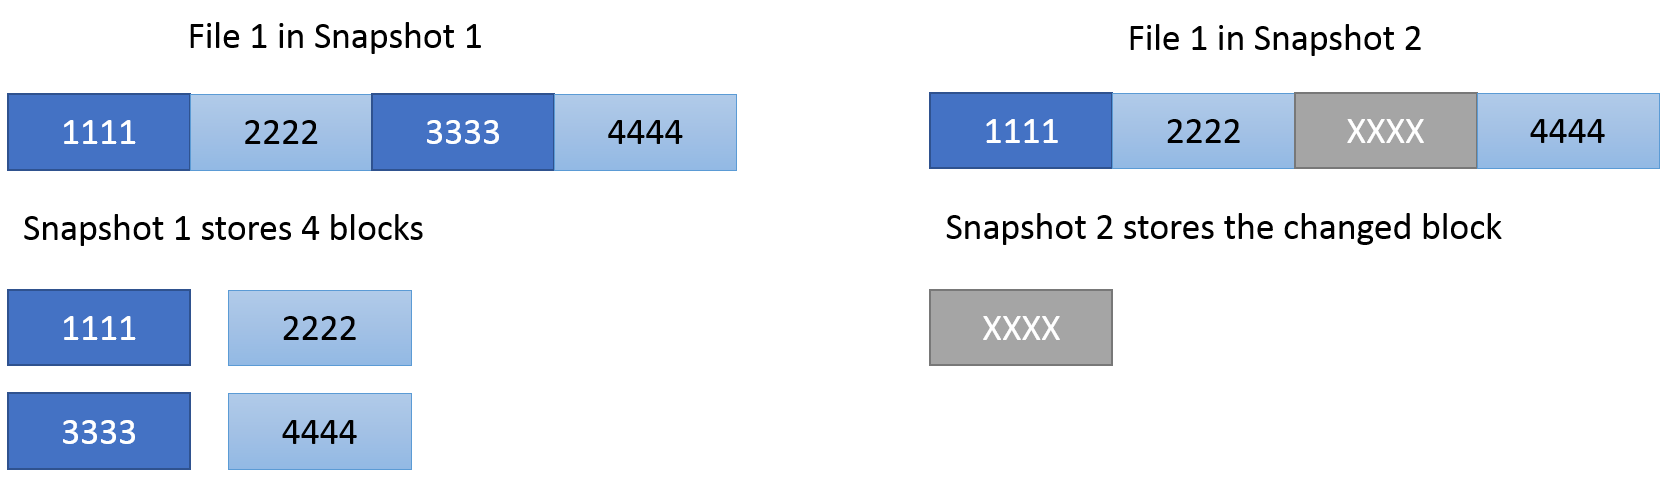
\includegraphics[width=0.8\textwidth]{Chapter-4/figs/fig4.png}
\caption{Classic Copy-on-Write}
\label{fig:classic_cow}
\end{figure}

    However, this is not always ideal. In many use cases, like insertion or deletion, a write operation only affects a few bytes instead of a whole block. But a classic file system will rewrite all successor blocks in these scenarios. A classic snapshot system will make a copy for all successor blocks despite the fact that only very few bytes are changed. The following \fref{fig:issue_classic_cow} addresses this issue. In this example, a byte is inserted into the file at offset 8. In classical copy-on-write snapshot system, two successor blocks are treated as changed blocks and will be copied. However, the data in those blocks did not change. They just got moved one byte forward. In the figure we also demonstrate a potentially better approach.

\begin{figure}[t]
\centering
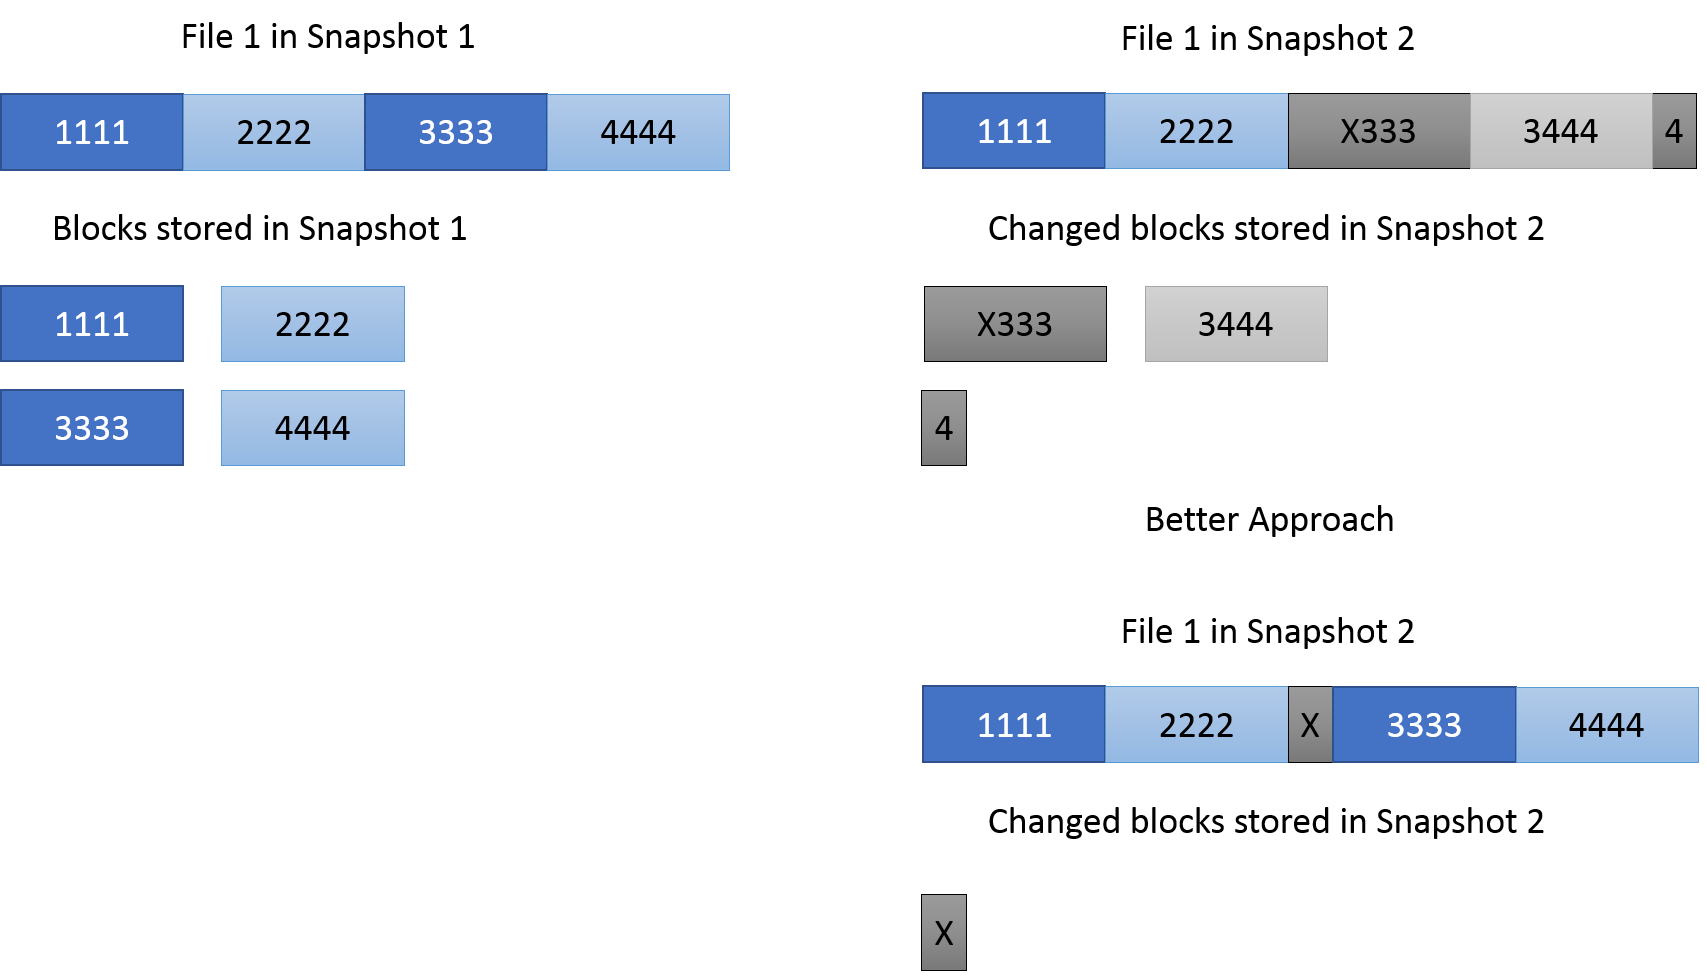
\includegraphics[width=0.8\textwidth]{Chapter-4/figs/fig5.png}
\caption{Issue in Classic Copy-on-Write}
\label{fig:issue_classic_cow}
\end{figure}
 
    To solve this problem, we have to let the file system be aware of the true intention of the end user. This is not straight forward because the POSIX standard uses only one file system call to handle all kinds of modification to a file. The only function of this file system call is to rewrite a part of a file.
    
    If a user program intends to insert a byte right in the middle of the file, the file system will receive a set of write calls to rewrite all later blocks in order to move the original data 1 byte forward. The same behavior can also be observed when the user program tries to rewrite the latter half of the file. It is difficult for the file system to distinguish these two scenario. Access patterns can be used to provide some clew of the intention of an operation (i.e., an insertion usually results in a truncate call followed by a series of write() calls), but it is not an ideal solution as it depends on how the user program behaves. Therefore, our major challenge is to identify the true intention of a write operation, whether should be an insertion or a complete rewrite. Next chapter, we will show how to accomplish this goal by using the rsync algorithm \cite{rsync_alg}.

\begin{figure}[t]
\centering
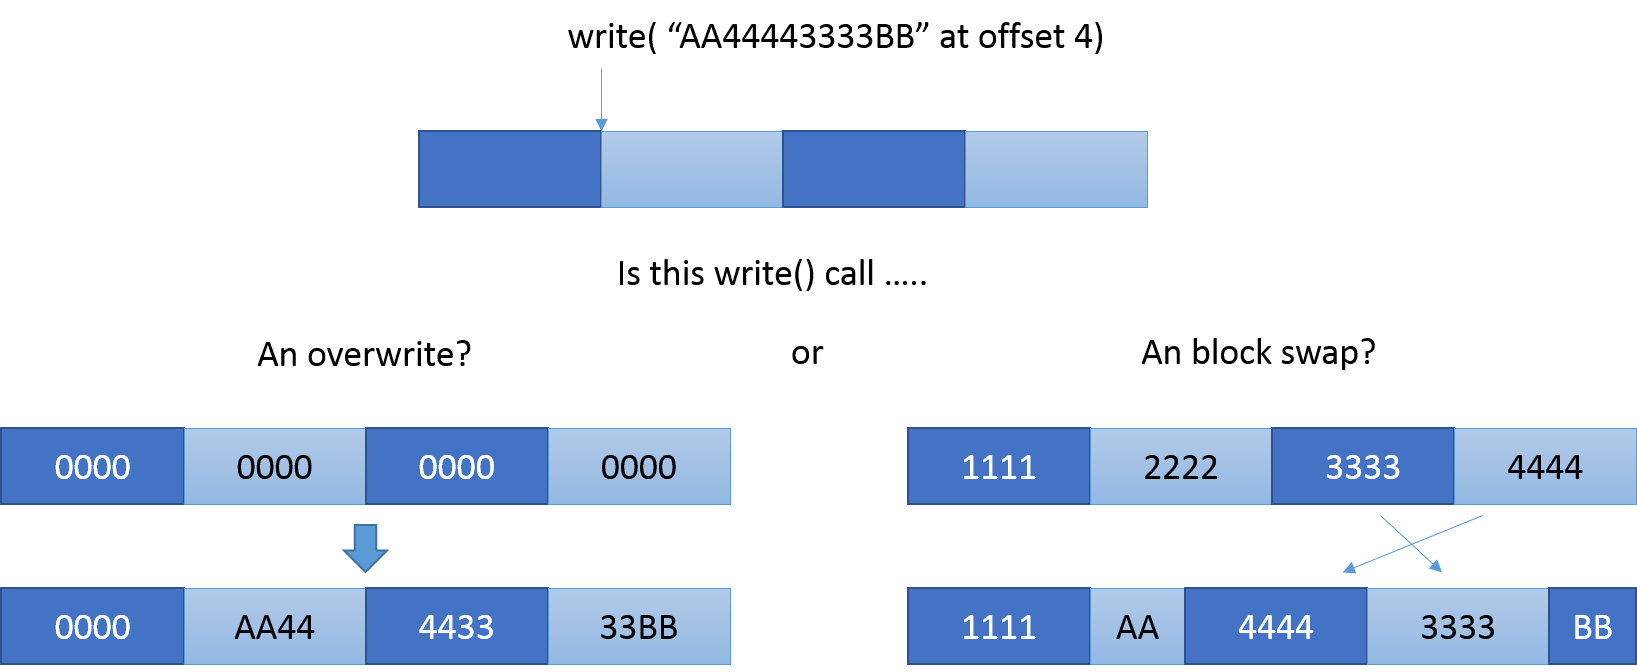
\includegraphics[width=0.8\textwidth]{Chapter-4/figs/fig6.png}
\caption{Identify the Intention of Write Operations}
\label{fig:write_intention}
\end{figure}

\subsection{The rsync algorithm}

    As discussed in the previous section, in order to identify duplications in a better way, we need to have a mechanism to compare the data to be written into the file and the original data. The rsync algorithm was originally designed for the efficient update of data over a high latency and low bandwidth link. Compared to the brute force search or string search algorithms, rsync algorithm is much faster in practice and requires less data exchange between the remote server and local machine. These features make it suitable for a distributed file system. Because either a time consuming file system or a high bandwidth consumption file system will become a bottleneck in the operating system.

    The basic flow of the original rsync algorithm is to split the remote file into blocks of length $S$, calculate their rolling checksum and then send them to the local machine. The local machine will search through the local file to find all blocks of length $S$ (at any offset, not just multiples of $S$) that matches the received rolling checksum. This can be done in a single pass very quickly since the rolling checksum algorithm only requires $O(1)$ time to compute the checksum at offset k if the checksum at offset $k-1$ is given.

\subsection{Enhancing the Space Efficiency}

    The Kabi File System uses the rsync algorithm to enhance the space efficiency of snapshots. It assumes that in most cases two different versions of the same file will share part of their data.

    In the Kabi File System, a section object in a file node contains not only the reference to the corresponding block, but also contains the rolling checksums of the block data. Before flushing the write buffer, the local machine will calculate the rolling checksums of data blocks at all possible offsets. The file system will compare these rolling checksums with those fetched from remote. If a match is found, the file system will then double check their SHA-1 hash to confirm that it is indeed a duplication.
    
    Once all data blocks have been examined, the local machine will send IDs of duplicated blocks and all remaining data back to the remote server.


\begin{figure}[t]
\centering
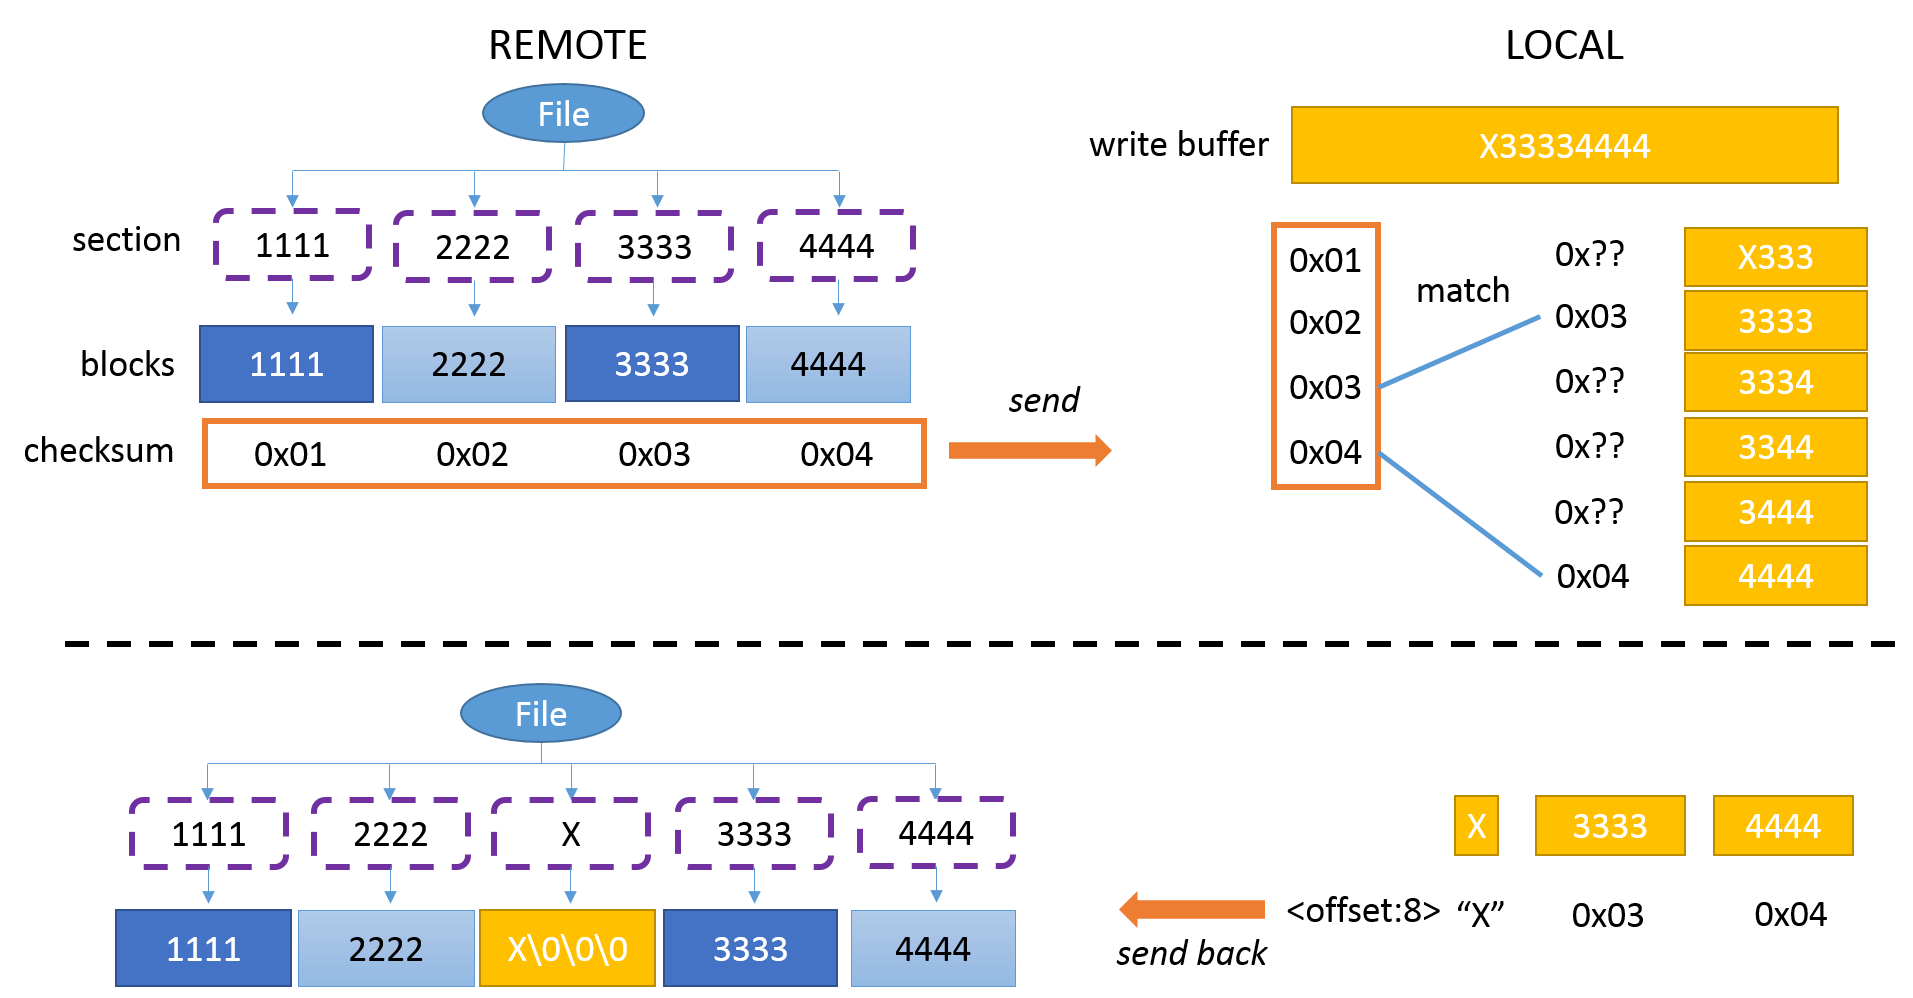
\includegraphics[width=0.9\textwidth]{Chapter-4/figs/fig25.png}
\caption{Using Rsync to Find Unchanged Blocks}
\label{fig:rsync}
\end{figure}

    During this process, the computational overhead is only the calculation and matching of rolling checksums. An important property of rolling checksum algorithm is that successive values can be computed in $O(1)$ time. Thus it ensures that all rolling checksums can be calculated in $O(n)$ time. In contrast, the benefits is a significant decrease in both network flow and remote storage when there exists data duplication.

\section{Conclusion}

   In this chapter, we present the basic idea of this snapshot system and discuss some implementation details of the snapshot subsystem in the Kabi File System. We demonstrated our efforts to make the snapshot system efficient in space usage. We also introduced the rsync algorithm to improve the snapshot system and the network performance.

